\documentclass[14pt]{extarticle}
\usepackage{knu-fcc-style}
\usepackage{graphicx}
\usepackage{booktabs}

\begin{document}

\KNUTitlePageMake[
  type={Звіт до лабораторної роботи №2},
  specialty={122 Комп'ютерні науки},
  title={Паралельне MPI-моделювання теплоперенесення на STL-меші},
  studentInfo={Виконав студент}, student={ПІБ студента},
  studentSignature={false}, supervisorSignature={false}, year={2026}
]

\KNUUnnumberedSection{Реферат}
Робота присвячена паралельному моделюванню поширення теплової енергії на трикутній поверхні STL. Температура пов'язується з полігонами, а передача енергії визначається графом сусідства за спільними ребрами. Реалізацію виконано мовою Python із застосуванням \texttt{mpi4py}, Slurm та чотирьох MPI-процесів.

\KNUKeywords{MPI, SLURM, STL, МЕШ, ТЕПЛОПЕРЕНЕСЕННЯ, ПАРАЛЕЛЬНІ ОБЧИСЛЕННЯ}
\KNUContents

\KNUUnnumberedSection{Вступ}
Метою роботи є реалізація моделі теплоперенесення на поверхні трикутного меша та дослідження її масштабування на навчальному Slurm-кластері. Використано Stanford Dragon, спрощений з 871\,414 до 115\,447 полігонів. Його розбито між MPI-процесами просторово; температури граничних полігонів передаються через ghost-зони.

\section{Математична модель та реалізація}
Для полігона $i$ використано явну схему теплопровідності
\begin{equation}
 C_i\frac{dT_i}{dt}=\sum_{j\in N(i)}K_{ij}(T_j-T_i),
 \qquad T_i^{n+1}=T_i^n+\frac{\Delta t}{C_i}\sum_{j\in N(i)}K_{ij}(T_j^n-T_i^n).
\end{equation}
Тут $C_i=\rho c h A_i$, а $K_{ij}=kL_{ij}/d_{ij}$. Сусідніми є полігони, що мають спільне ребро. Центральний полігон підтримується при температурі 500, а зовнішні ребра вважаються теплоізольованими.

У кожному кроці MPI-процеси неблокувально обмінюються температурами лише тих полігонів, що межують з іншими піддоменами. Для OpenMPI використано інтерфейс \texttt{eth1} кластерної мережі 192.168.56.0/24, а не NAT-інтерфейс Vagrant.

\section{Експеримент}
Виконано три повтори для $N=1,2,3,4$ MPI-процесів і 300 часових кроків. Окремо виміряно читання меша, побудову суміжності, MPI-розбиття та теплообмін.

\begin{table}
\caption{Медіанні результати теплообміну Stanford Dragon}
\centering
\begin{tabular}{rrrrr}
\toprule
$N$ & Кроків & Час, с & Speedup & Efficiency, \% \\
\midrule
1 & 300 & 67.664 & 1.000 & 100.00 \\
2 & 300 & 40.512 & 1.670 & 83.51 \\
3 & 300 & 31.849 & 2.125 & 70.82 \\
4 & 300 & 26.512 & 2.552 & 63.81 \\
4 & 12\,000 & 624.711 & --- & --- \\
\bottomrule
\end{tabular}
\label{tab:benchmark}
\end{table}

\begin{table}
\caption{Окремо виміряні підготовчі задачі}
\centering
\begin{tabular}{lrr}
\toprule
Режим & $T(1)$, с & $T(4)$, с \\
\midrule
Завантаження меша & 0.650 & 0.838 \\
Сусідство полігонів & 10.028 & 10.478 \\
MPI-розбиття & 10.012 & 10.375 \\
\bottomrule
\end{tabular}
\end{table}

\section{Візуалізація та аналіз}
Рисунок~\ref{fig:temperature-n4} показує результат окремого візуалізаційного розрахунку на 12\,000 часових кроків із гарячою областю, а не одним полігоном. Цей запуск на чотирьох MPI-процесах завершився за 624.711~с; він наведений окремим рядком у таблиці~\ref{tab:benchmark} і не входить до обчислення Speedup, бо не має серії повторів для $N=1$. Рисунки~\ref{fig:mpi-partition}--\ref{fig:adjacency} демонструють декомпозицію меша, ghost-зони й зв'язки сусідства. Значення $S(4)=2.552$ підтверджує прискорення, а зниження ефективності до 63.81\% пояснюється MPI-обмінами та накладними витратами запуску у віртуалізованому кластері. Режими читання, суміжності та розбиття не мають прискорення, оскільки їхню підготовчу частину навмисно виконує rank 0.

% Generated from the 4-node Stanford Dragon visualization run, job 337.
\begin{figure}[htbp]
  \centering
  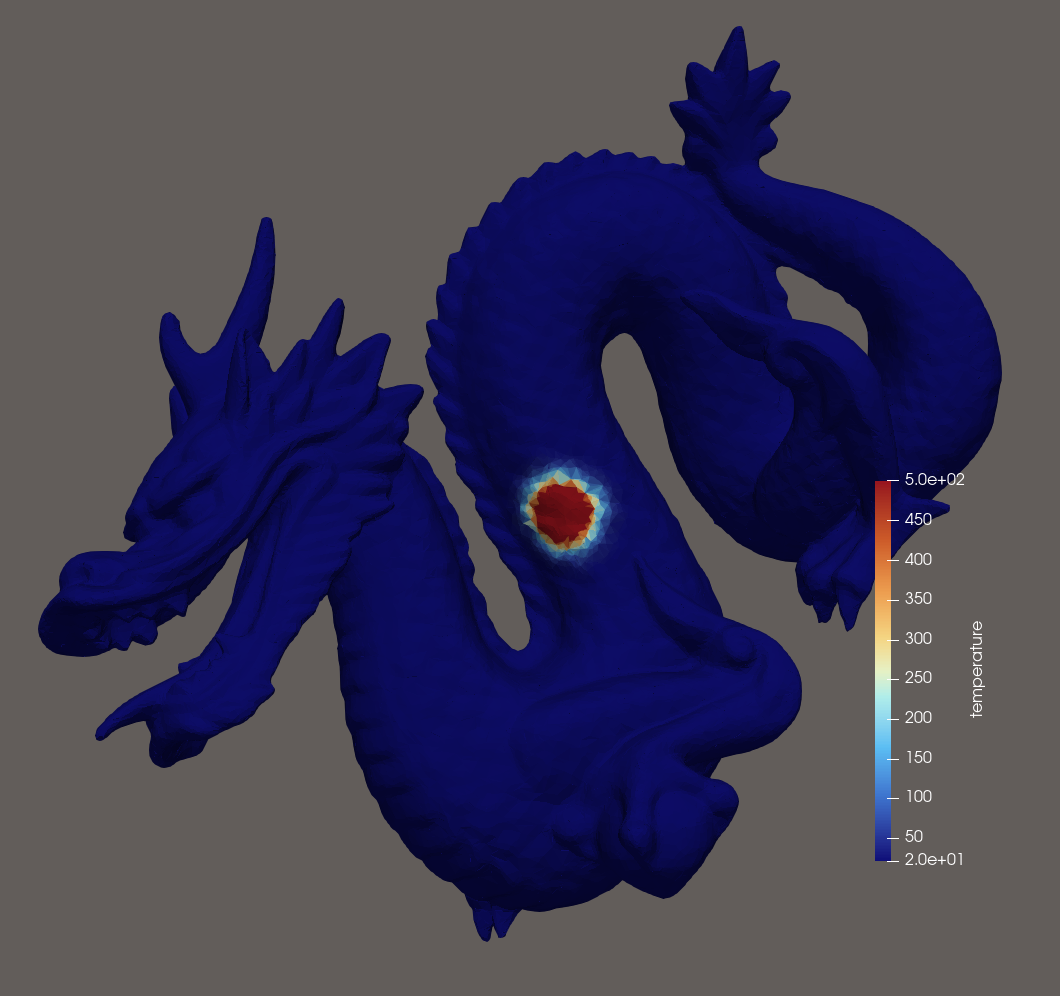
\includegraphics[width=0.88\linewidth]{figures/temperature_paraview.png}
  \caption{Розподіл температури на STL-поверхні Stanford Dragon після 12\,000 часових кроків, візуалізований у ParaView.
  Меш містить 115\,447 трикутних полігонів; температура кольором відповідає
  атрибуту полігона, а область джерела підтримується на рівні $500$.}
  \label{fig:temperature-n4}
\end{figure}

\begin{figure}[htbp]
  \centering
  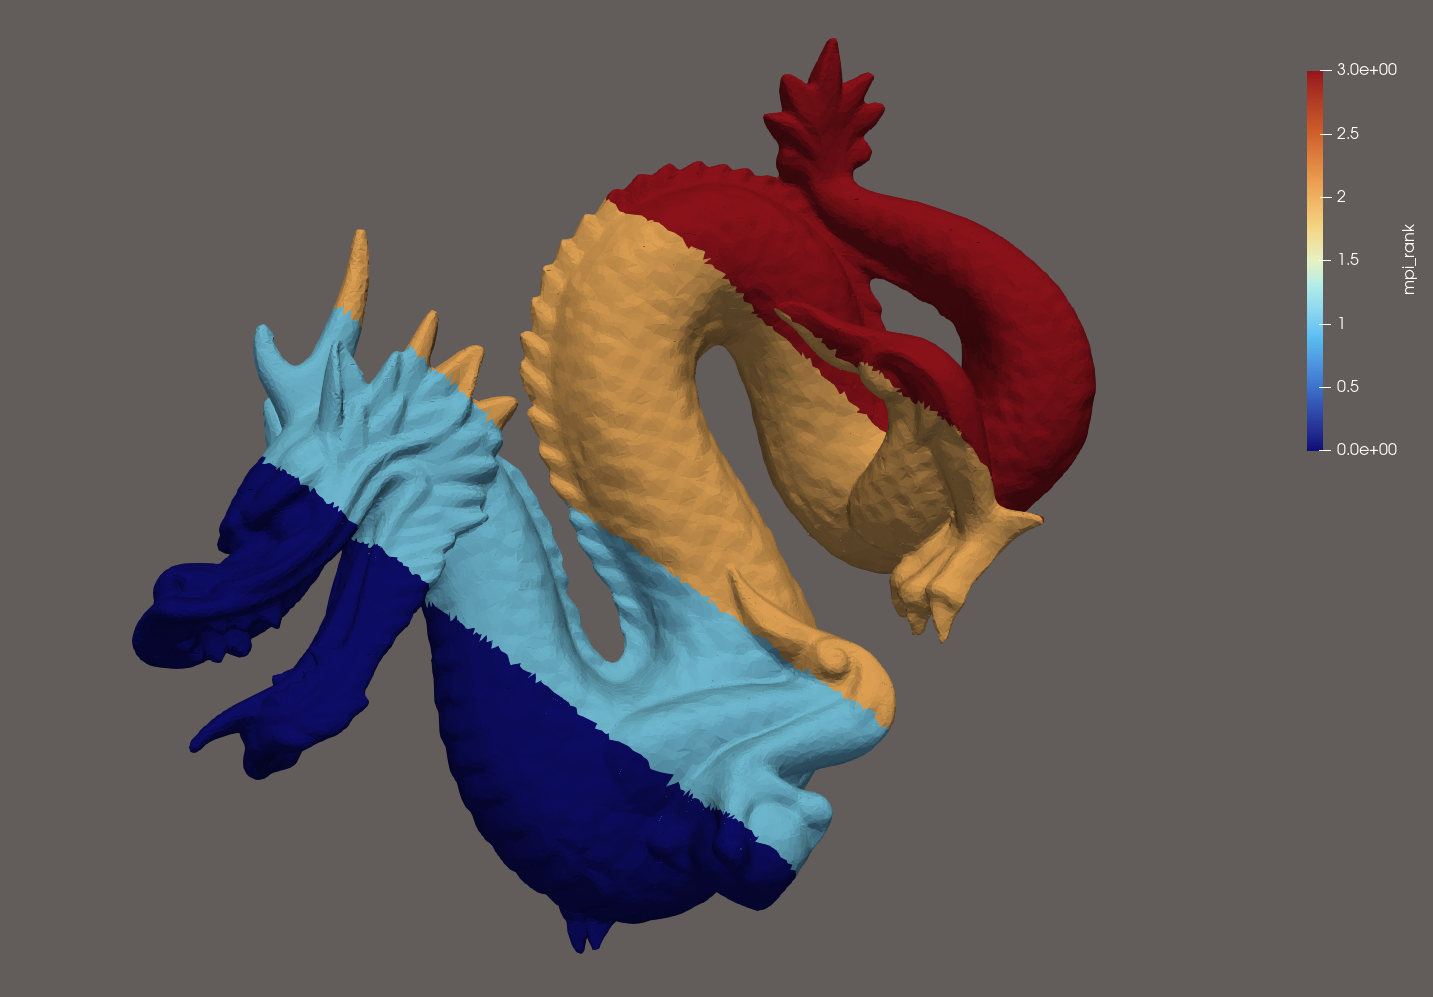
\includegraphics[width=0.48\linewidth]{figures/partition_paraview.png}
  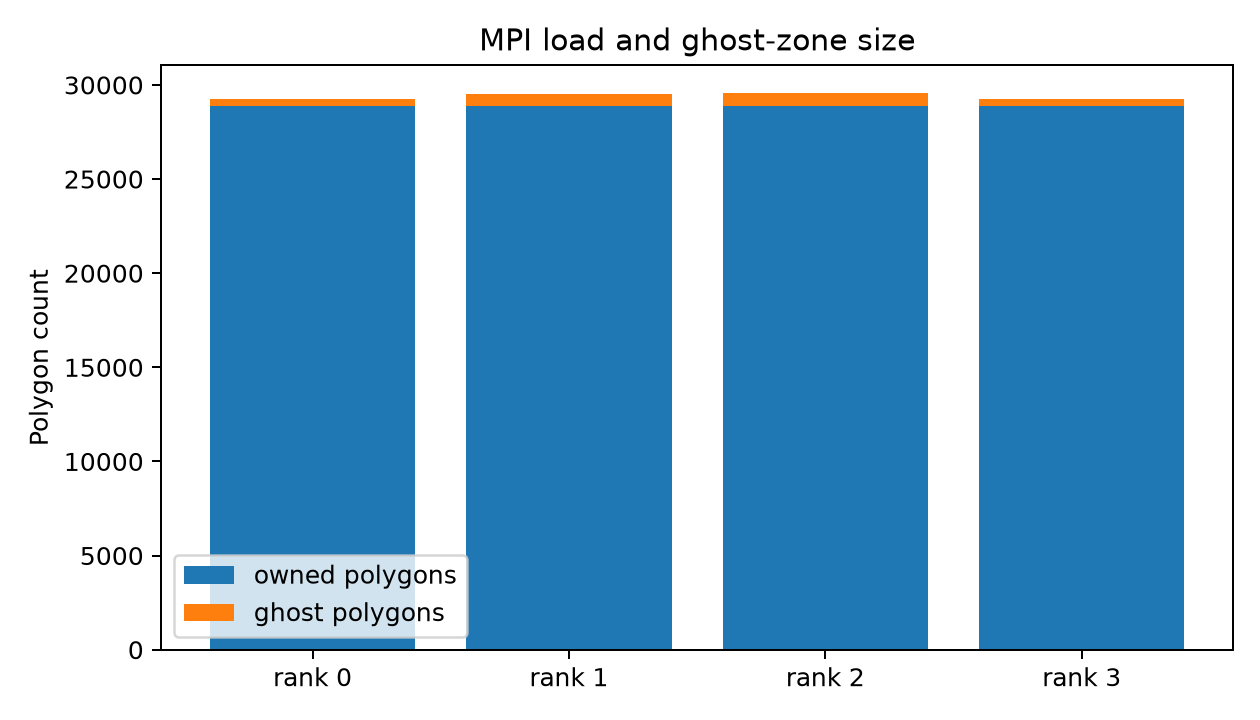
\includegraphics[width=0.48\linewidth]{figures/load_ghost_distribution.png}
  \caption{Просторове розбиття меша між чотирма MPI-процесами у ParaView та
  кількість власних і ghost-полігонів кожного процесу.}
  \label{fig:mpi-partition}
\end{figure}

\begin{figure}[htbp]
  \centering
  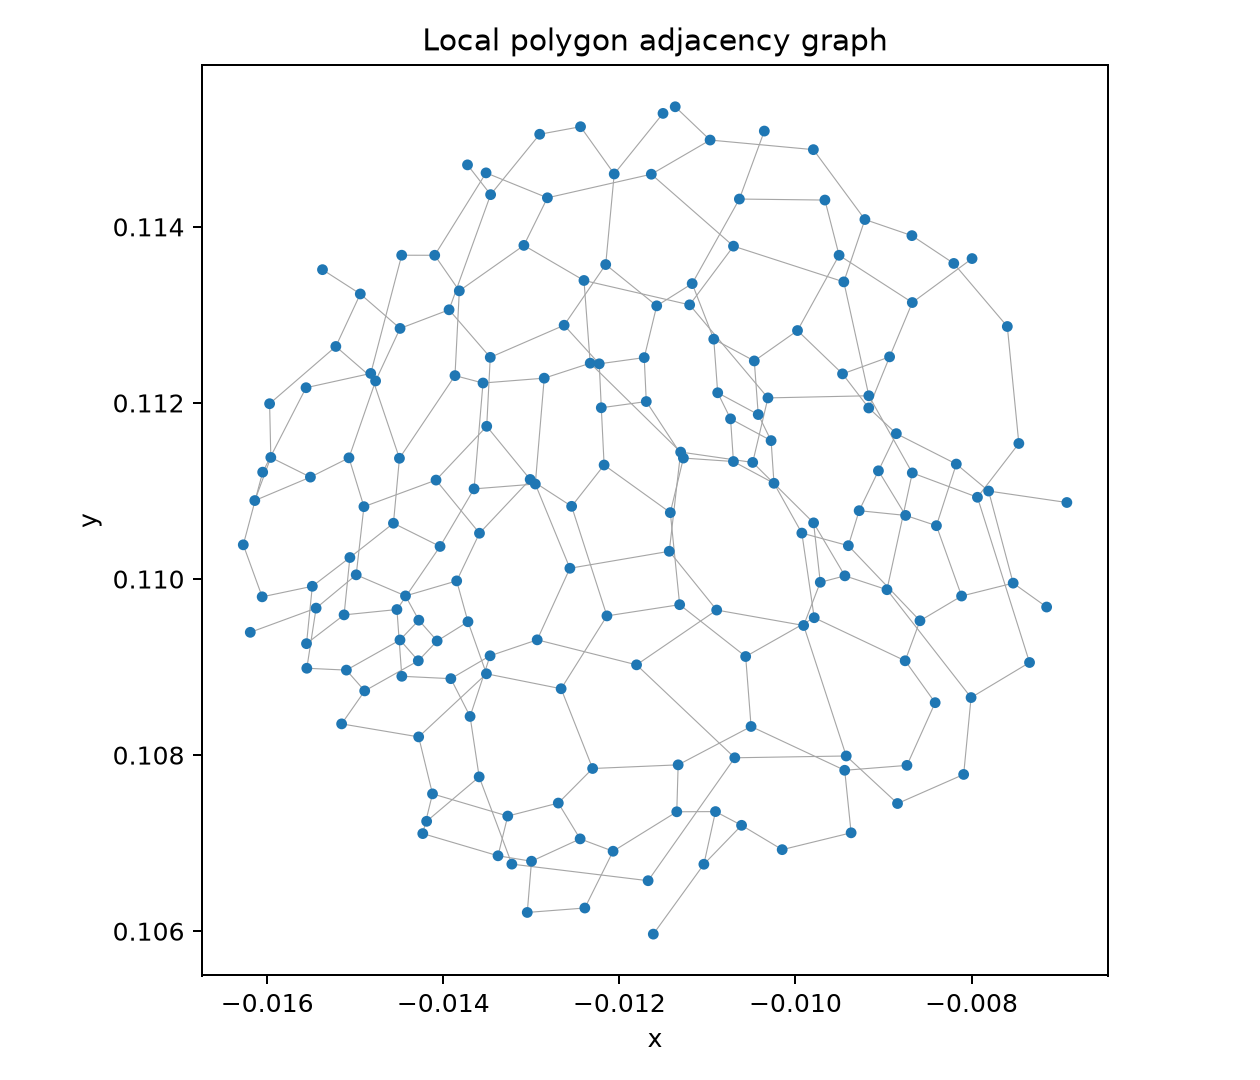
\includegraphics[width=0.62\linewidth]{figures/adjacency_graph.png}
  \caption{Локальний фрагмент графа сусідства трикутних полігонів.
  Лінія означає наявність спільного ребра, колір вершини --- MPI rank.}
  \label{fig:adjacency}
\end{figure}

\begin{figure}[htbp]
  \centering
  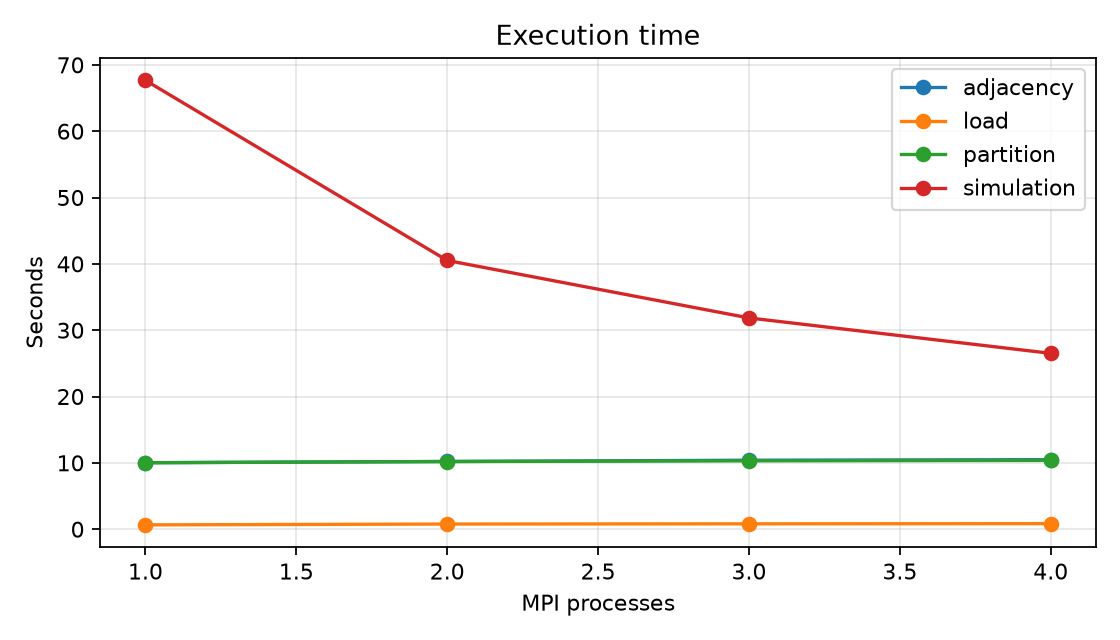
\includegraphics[width=0.48\linewidth]{figures/execution_time.png}
  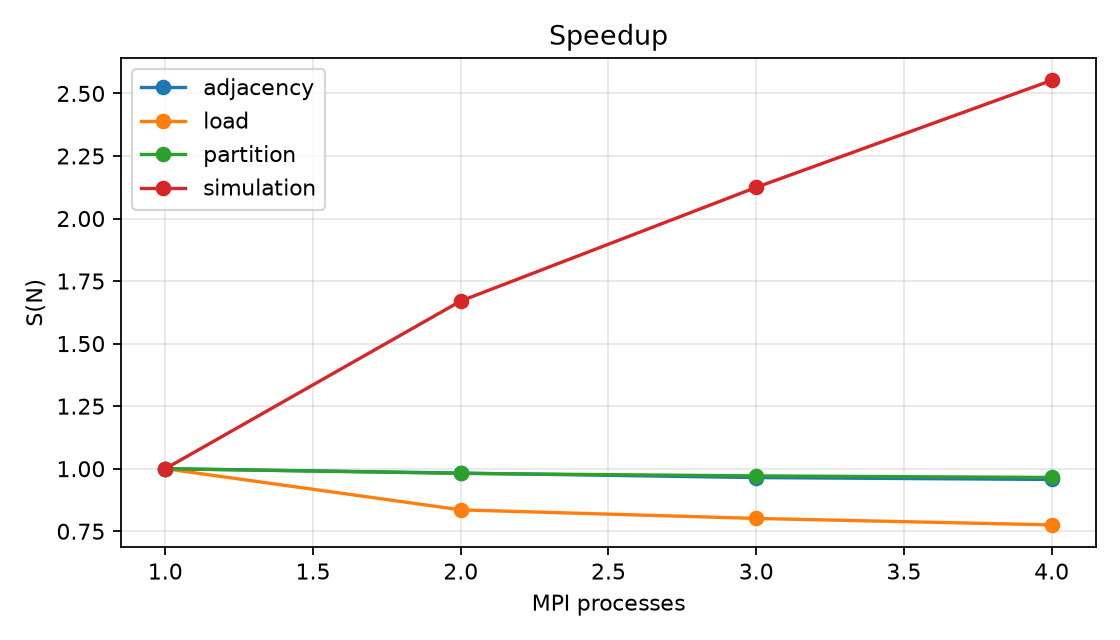
\includegraphics[width=0.48\linewidth]{figures/speedup.png}
  \caption{Медіанний час виконання та прискорення окремих режимів для Stanford Dragon,
  300 часових кроків і трьох повторів кожної конфігурації.}
  \label{fig:scaling}
\end{figure}


\KNUUnnumberedSection{Висновки}
Реалізовано MPI-модель теплоперенесення на STL-поверхні Stanford Dragon з атрибутом температури, графом суміжності полігонів і ghost-обміном на межах піддоменів. Усі 48 запусків benchmark завершилися успішно. На чотирьох процесах медіанний час моделювання зменшився з 67.664~с до 26.512~с. Результати також експортовано у VTK для інтерактивної візуалізації температури та MPI-розбиття в ParaView.

\begin{thebibliography}{9}
\bibitem{mpi} MPI Forum. MPI: A Message-Passing Interface Standard. \url{https://www.mpi-forum.org/}.
\bibitem{slurm} Slurm Workload Manager Documentation. \url{https://slurm.schedmd.com/}.
\bibitem{numpy-stl} numpy-stl Documentation. \url{https://numpy-stl.readthedocs.io/}.
\end{thebibliography}

\end{document}
